\documentclass{article}

\usepackage[english]{babel}
\usepackage[letterpaper,top=2cm,bottom=2cm,left=3cm,right=3cm,marginparwidth=1.75cm]{geometry}

% Useful packages
\usepackage{amsmath}
\usepackage{graphicx}
\usepackage{float}
\usepackage[colorlinks=true, allcolors=blue]{hyperref}

\title{Tourism Activity Analysis Using Supervised Machine Learning}
\author{Motelică Sandu}

\begin{document}
\maketitle

\section{Introduction}
The purpose of this project is to analyze a tourism dataset sourced from the Kaggle repository (\url{https://www.kaggle.com/datasets/umeradnaan/tourism-dataset}), focusing on the profitability and popularity of six tourism activity categories (\textit{Nature, Historical, Cultural, Beach, Adventure, Urban}) across seven countries. Using both data visualization techniques and supervised machine learning models (e.g., \textit{ID3 Trees, Na\"{i}ve Bayes, Optimal Bayes, Linear Regression,  k-Nearest Neighbors (kNN)}, and \textit{AdaBoost Trees} ), this study aims to rank these categories based on their revenue potential and visitor metrics.

Key objectives of this analysis include:
\begin{itemize}
    \item Understanding the data through exploratory analysis, identifying key patterns and correlations.
    \item Preprocessing the data to prepare it for machine learning models, including feature encoding and discretization.
    \item Developing a decision-making model to rank activity categories based on profitability indicators such as \textit{Revenue} and \textit{Revenue per Visitor}.
\end{itemize}

This work is intended for educational purposes and demonstrates the application of supervised learning in real-world datasets.

\section{Data Understanding and Exploration}
The dataset provides insights into various tourism activities across seven countries and includes the following attributes:

\begin{itemize}
    \item \textbf{Location}: A unique identifier for each record.
    \item \textbf{Country:} The country where the activity is located.
    \item \textbf{Category:} The activity type, with six possible categories:
          \textit{Nature, Historical, Cultural, Beach, Adventure, Urban}.
    \item \textbf{Visitors:} The total number of visitors engaging in the activity.
    \item \textbf{Rating:} The average rating provided by visitors for the activity.
    \item \textbf{Revenue:} The total revenue generated by the activity.
    \item \textbf{Accommodation\_Available:} A binary indicator of whether accommodation is provided (\textit{Yes/No}).
\end{itemize}

This dataset offers a mix of numerical and categorical data, requiring both descriptive analysis and feature engineering to extract meaningful insights.

\subsection{Exploratory Data Analysis}
Exploratory Data Analysis serves as the foundation for understanding the dataset. In this section, we analyze visitor trends, revenue distributions, and correlations between numerical attributes. Insights from these analyses guide the feature engineering and model-building process.

\subsubsection{Revenue and Visitor Trends Across Categories}
Figures~\ref{fig:visitors_distribution} and~\ref{fig:revenue_distribution} illustrate the distribution of visitors and revenue for the six activity categories. Key observations include:
\begin{itemize}
    \item \textbf{Visitor Patterns:} The number of visitors is relatively similar across categories, with median values clustering around 400,000 to 600,000. However, certain categories like \textit{Adventure} exhibit a wider range, suggesting both niche and highly popular activities.
    \item \textbf{Revenue Distribution:} Revenue medians also show consistency, but variability within categories (e.g., \textit{Nature} and \textit{Beach}) indicates significant revenue outliers, likely due to high-value activities.
    \item \textbf{Category Analysis:} Categories such as \textit{Urban} and \textit{Cultural} appear to have tighter distributions, suggesting more consistent performance across activities.
\end{itemize}


\begin{figure}[H]
    \centering
    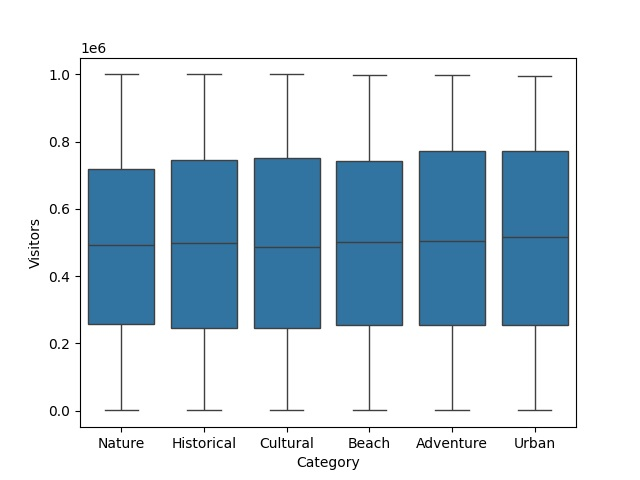
\includegraphics[width=0.6\textwidth]{visitors_distribution.jpg}
    \caption{Visitors Distribution Across Categories}
    \label{fig:visitors_distribution}
\end{figure}

\begin{figure}[H]
    \centering
    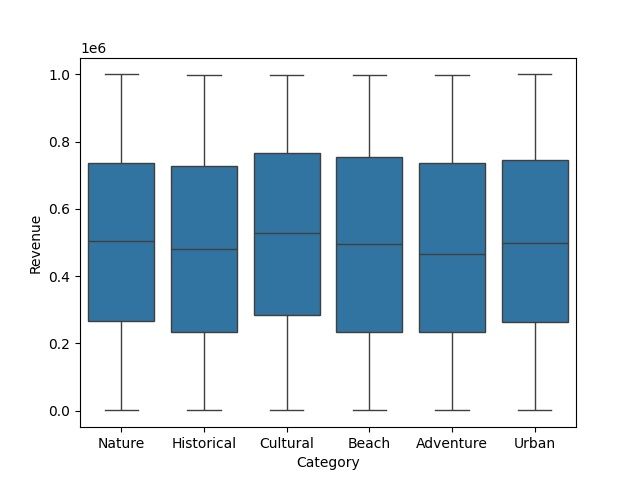
\includegraphics[width=0.6\textwidth]{revenue_distribution.jpg}
    \caption{Revenue Distribution Across Categories}
    \label{fig:revenue_distribution}
\end{figure}


\subsubsection{Correlation Analysis of Numerical Features}
Figure~\ref{fig:correlation_heatmap} presents the correlation heatmap for numerical attributes, revealing the following:
\begin{itemize}
	\item \textbf{General Observations on Correlation:} The lack of strong correlations between most attributes underscores the diverse nature of tourism activities, where various factors independently influence outcomes. 
    \item \textbf{Revenue and Visitors:} A weak positive correlation (\textit{correlation coefficient = 0.01}) suggests that while more visitors generally increase revenue, the effect is marginal.
    \item \textbf{Revenue per Visitor:} A weak negative correlation with visitor count (\textit{correlation coefficient = -0.24}) highlights the importance of niche activities, which may generate high returns despite fewer visitors.
    \item \textbf{Rating and Visitors:} There is minimal correlation, implying that visitor numbers do not significantly influence activity ratings.
\end{itemize}

\begin{figure}[H]
    \centering
    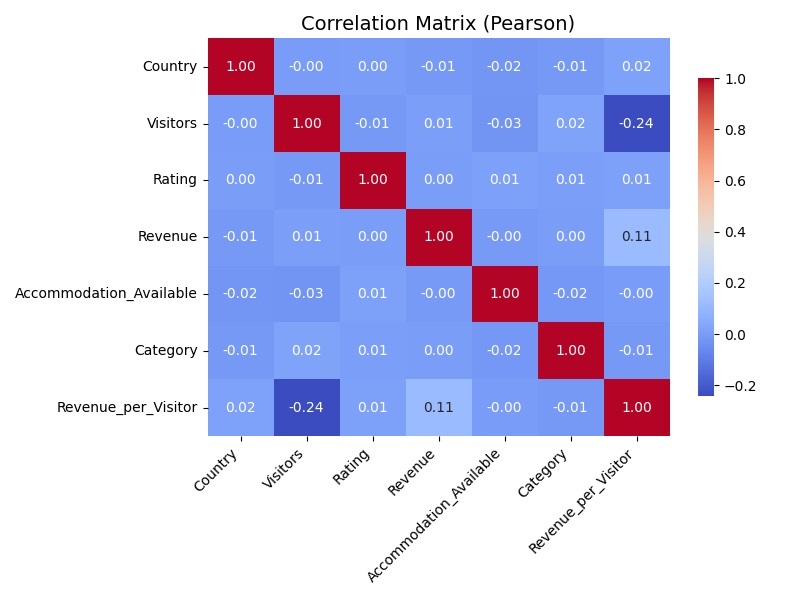
\includegraphics[width=0.8\textwidth]{correlation_matrix.jpg}
    \caption{Correlation Heatmap of Numerical Attributes}
    \label{fig:correlation_heatmap}
\end{figure}

\subsubsection{Revenue by Country and Category}
Figure~\ref{fig:revenue_by_country_category} shows the revenue distribution for six activity categories across seven countries. Key insights include:

\begin{itemize}
    \item \textbf{Country-Specific Trends:} 
        - Egypt dominates in \textit{Urban} activities, while India and China excel in \textit{Cultural} tourism.
        - France shows consistently lower revenue across categories.

    \item \textbf{Category Highlights:}
        - \textit{Beach} activities generate the highest revenue in India, while \textit{Nature} performs strongly in Australia and Brazil.
        - \textit{Cultural} activities show stable revenue trends across all countries, indicating universal appeal.

\end{itemize}

These trends underline the importance of tailoring tourism strategies to each country’s strengths and revenue drivers.

\begin{figure}[H]
    \centering
    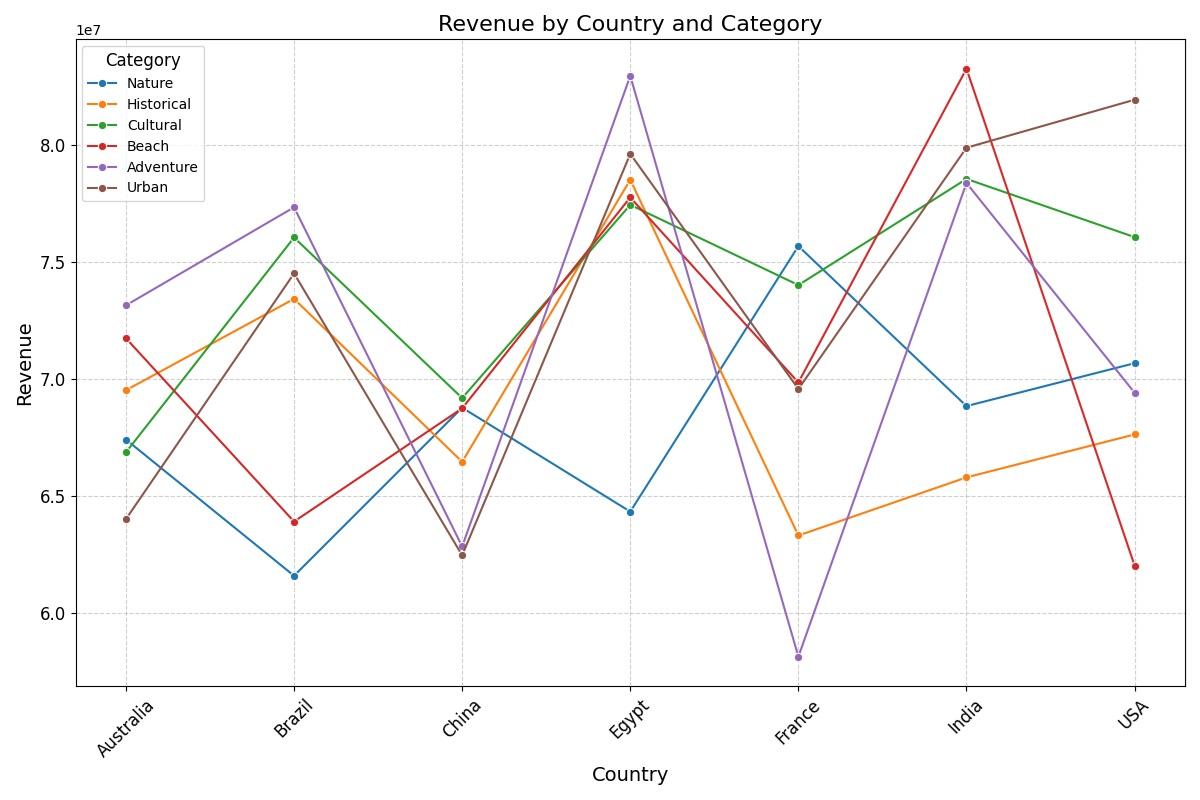
\includegraphics[width=0.8\textwidth]{category_country_distribution.jpg}
    \caption{Revenue by Country and Category}
    \label{fig:revenue_by_country_category}
\end{figure}


\subsection{Conclusion}
The exploratory analysis underscores the importance of advanced machine learning models to capture non-linear relationships between features. Weak negative correlation
between revenue per visitor and total visitors underscores the potential value of niche, high-value
activities, which may yield better returns despite lower attendance.

\section{Experimental results and theoretical analysis}


In this section, we evaluate and analyse the performance of various supervised machine learning algorithms applied to the tourism dataset. The goal is to determine the most effective approach for predicting the profitability of tourism activity categories based on the dataset's attributes. The algorithms tested include \textit{ID3 Trees, Na\"{i}ve Bayes, k-Nearest Neighbors (kNN), Linear Regression}, and \textit{AdaBoost}. Each algorithm is assessed based on its ability to generate accurate predictions, with results compared across different countries and experimental configurations.

\subsection{Results for Na\"{i}ve Bayes}

To begin, we present the results of experiments conducted using the \textit{Na\"{i}ve Bayes} algorithm. This probabilistic classifier assumes that features are independent, which is not entirely true for this dataset but provides a useful baseline for comparison. Two approaches were tested:
\begin{itemize}
    \item In the \textbf{first approach}, the model used three attributes: \textit{Visitors, Rating}, and \textit{Accommodation}.
    \item In the \textbf{second approach}, three additional engineered features were included: \textit{Revenue per Visitor(provides an indicator of how much revenue is generated on average per visitor), Log of Visitors(reduces the skewness of the Visitors data, especially if there are activities with very large or very small visitor counts. It helps stabilize variance and improves the performance)}, and \textit{Log of Revenue(reduces the impact of large outliers in the Revenue attribute, enabling the algorithm to better handle data with large ranges)}.
\end{itemize}

The target variable for our analysis was the \textit{Category} of tourism activities, which was encoded for use in the classification model. The dataset was filtered for each country individually and  was split into an 80\%-20\% training and testing ratio, with the training set used to fit the \textit{Na\"{i}ve Bayes} model and the testing set employed to evaluate its accuracy. The dataset was split in such a way so every category to be found in both datasets in the given proportions. 80-20 report was selected in order to have balanced datasets, otherwise the test set could have different proportion for category entries, they even can miss some categories depending on how the data was splitted.

For revenue calculation, the predicted categories obtained from the \textit{Na\"{i}ve Bayes} model were first converted back to their original labels using the inverse transform of the \textit{LabelEncoder}. The corresponding \textit{Revenue} values for the test dataset were then assigned by matching the indices of the test data with the original dataset. This allowed each predicted category to be associated with its actual revenue value from the dataset. The revenue values were subsequently grouped by the predicted categories, and the average revenue for each category was computed. This average revenue served as a basis for ranking the categories, with higher average revenue indicating a higher rank.



Table~\ref{tab:naive_bayes_results} summarizes the accuracy of the \textit{Na\"{i}ve Bayes} model across the seven countries in the dataset for both approaches.

\begin{table}[h!]
    \centering
    \begin{tabular}{|c|c|c|}
        \hline
        \textbf{Country} & \textbf{Accuracy (First Approach)} & \textbf{Accuracy (Second Approach)} \\ \hline
        India & 16.67\% & 17.22\% \\
        USA & 12.94\% & 17.06\% \\
        Brazil & 15.86\% & 17.48\% \\
        France & 12.09\% & 22.21\% \\
        Egypt & 15.30\% & 18.03\% \\
        China & 9.88\% & 17.28\% \\
        Australia & 13.86\% & 17.47\% \\ \hline
    \end{tabular}
    \caption{Na\"{i}ve Bayes model accuracy across countries for the two approaches.}
    \label{tab:naive_bayes_results}
\end{table}

The results indicate that the second approach, which includes engineered features, consistently outperforms the first approach. This improvement is attributed to the inclusion of additional features, which provide more informative inputs for the classifier, adding an attribute that correlates 2, helps in this case. However, the overall accuracy remains relatively low, reflecting the limitations of the \textit{Na\"{i}ve Bayes} algorithm in handling datasets where attributes are not truly independent.

\subsection{Optimal Bayes}
The \textit{Optimal Bayes Classifier} represents the theoretical upper bound of classification performance, as it relies on the true posterior probabilities of the target classes. However, in practice, it cannot be directly applied because the true distributions of the data are generally unknown. Accurately estimating these probabilities is challenging, particularly when the data exhibits high dimensionality, complex relationships, or limited sample sizes.

\subsection{k-Nearest Neighbors (kNN)}

To analyze the dataset and predict revenue rankings among tourism categories, the \textit{k-Nearest Neighbors (kNN)} algorithm was employed. The implementation included preprocessing, hyperparameter tuning, and evaluation to achieve optimal results. Below, we outline the steps undertaken:

\subsubsection{Data Preprocessing}

The dataset was filtered by country to ensure predictions were specific to each region. The following preprocessing steps were applied:
\begin{itemize}
    \item \textbf{Categorical Encoding:} The categorical variables \textit{Category} and \textit{Accommodation Available} were encoded into numerical values using \textit{LabelEncoder}.
    \item \textbf{Feature Selection:} The features used for prediction included \textit{Visitors}, \textit{Rating}, and the encoded \textit{Accommodation Available}. The target variable was \textit{Revenue}.
    \item \textbf{Feature Scaling:} All numerical features were standardized using \textit{StandardScaler} to ensure equal importance in distance calculations during the kNN process.
\end{itemize}

\subsubsection{Hyperparameter Tuning}

To optimize the kNN model, a grid search was conducted over the following hyperparameters:
\begin{itemize}
    \item \textbf{Number of Neighbors (\textit{k}):} Values ranging from 1 to 20 were tested to find the optimal number of neighbors.
    \item \textbf{Weighting Scheme:} Both \textit{uniform} weighting (equal importance for all neighbors) and \textit{distance} weighting (closer neighbors have greater influence) were evaluated.
    \item \textbf{Distance Metric:} Three distance metrics (\textit{Euclidean}, \textit{Manhattan}, and \textit{Minkowski}) were considered to identify the most suitable measure for the data.
\end{itemize}

The grid search was implemented using \textit{GridSearchCV} with 5-fold cross-validation. The performance of each parameter combination was assessed using the \textit{R²} score, and the best-performing model was selected.

\subsubsection{Data Splitting and Evaluation}

The dataset for each country was split into training and test sets using an 80\%-20\% ratio. The training set was used to tune the hyperparameters, while the test set was used to evaluate the final model's performance. The evaluation metrics included:
\begin{itemize}
    \item \textbf{Mean Absolute Error (MAE):} The average absolute difference between predicted and actual revenue values.
    \item \textbf{Mean Squared Error (MSE):} The average squared difference between predicted and actual revenue values, penalizing larger errors more heavily.
    \item \textbf{R² Score:} The proportion of variance in the target variable explained by the model.
\end{itemize}

\subsubsection{Results}

The kNN model was successfully tuned and evaluated for each country. The best combination of hyperparameters and the resulting evaluation metrics provided insights into the model's performance and its ability to rank tourism categories effectively by revenue. Below are the detailed results for each country:

\begin{itemize}
    \item \textbf{India:}
    Best Parameters: \{\texttt{metric}: \texttt{manhattan}, \texttt{n\_neighbors}: 20, \texttt{weights}: \texttt{uniform}\} \\
    Mean Absolute Error (MAE): 250,002.99 \\
    Mean Squared Error (MSE): 84,212,093,157.66 \\
    R² Score: -0.07 \\

    \item \textbf{USA:}
    Best Parameters: \{\texttt{metric}: \texttt{euclidean}, \texttt{n\_neighbors}: 20, \texttt{weights}: \texttt{uniform}\} \\
    Mean Absolute Error (MAE): 266,012.43 \\
    Mean Squared Error (MSE): 92,470,942,379.95 \\
    R² Score: -0.03 \\

    \item \textbf{Brazil:}
    Best Parameters: \{\texttt{metric}: \texttt{euclidean}, \texttt{n\_neighbors}: 18, \texttt{weights}: \texttt{uniform}\} \\
    Mean Absolute Error (MAE): 248,417.03 \\
    Mean Squared Error (MSE): 85,347,637,019.66 \\
    R² Score: 0.01 \\

    \item \textbf{France:}
    Best Parameters: \{\texttt{metric}: \texttt{manhattan}, \texttt{n\_neighbors}: 20, \texttt{weights}: \texttt{uniform}\} \\
    Mean Absolute Error (MAE): 243,704.18 \\
    Mean Squared Error (MSE): 80,476,138,214.68 \\
    R² Score: 0.01 \\

    \item \textbf{Egypt:}
    Best Parameters: \{\texttt{metric}: \texttt{manhattan}, \texttt{n\_neighbors}: 17, \texttt{weights}: \texttt{uniform}\} \\
    Mean Absolute Error (MAE): 238,704.22 \\
    Mean Squared Error (MSE): 79,403,452,509.68 \\
    R² Score: -0.02 \\

    \item \textbf{China:}
    Best Parameters: \{\texttt{metric}: \texttt{euclidean}, \texttt{n\_neighbors}: 20, \texttt{weights}: \texttt{distance}\} \\
    Mean Absolute Error (MAE): 257,102.73 \\
    Mean Squared Error (MSE): 89,774,913,666.07 \\
    R² Score: -0.08 \\

    \item \textbf{Australia:}
    Best Parameters: \{\texttt{metric}: \texttt{manhattan}, \texttt{n\_neighbors}: 20, \texttt{weights}: \texttt{uniform}\} \\
    Mean Absolute Error (MAE): 247,923.57 \\
    Mean Squared Error (MSE): 84,585,949,807.37 \\
    R² Score: -0.08 \\
\end{itemize}

Overall, while the tuning process identified the optimal hyperparameters for each country, the evaluation metrics indicate challenges in accurately predicting revenue using the kNN model. The low and negative R² scores highlight the limitations of the model, possibly due to the inherent complexity of the dataset or lack of strong feature-target relationships.

\subsection{ID3 Decision Tree Implementation}
The \textit{ID3 Decision Tree} algorithm was employed to predict the most profitable activity categories. Two approaches were analyzed:
\begin{enumerate}
    \item A \textbf{baseline approach} using raw numerical features without discretization or hyperparameter optimization.
    \item An \textbf{enhanced approach} that included discretization of key features and optimization of hyperparameters for quantile binning.
\end{enumerate}
This section details the methodologies, results, and comparisons of both approaches across countries.

\subsubsection{Baseline Approach}
The baseline approach utilized the raw numerical features (\textit{Visitors, Rating, Revenue per Visitor}) without any feature discretization. Categorical attributes (\textit{Category, Accommodation}) were encoded using \textit{LabelEncoder}, and the dataset was split into 80\% training and 20\% testing data for each country.

\textbf{Results:} Table~\ref{tab:id3_baseline_results} summarizes the accuracy and revenue hierarchy predictions for each country using this approach.

\begin{table}[h!]
    \centering
    \begin{tabular}{|c|c|l|}
        \hline
        \textbf{Country} & \textbf{Accuracy} & \textbf{Top Revenue Categories (Baseline)} \\ \hline
        India & 15.00\% & Nature, Historical, Beach \\ 
        USA & 15.88\% & Nature, Cultural, Urban \\ 
        Brazil & 18.45\% & Cultural, Beach, Adventure \\ 
        France & 11.63\% & Urban, Cultural, Nature \\ 
        Egypt & 21.31\% & Cultural, Historical, Urban \\ 
        China & 16.05\% & Adventure, Nature, Beach \\ 
        Australia & 18.67\% & Historical, Nature, Cultural \\ \hline
    \end{tabular}
    \caption{ID3 Baseline Results Across Countries}
    \label{tab:id3_baseline_results}
\end{table}

\textbf{Analysis:}
\begin{itemize}
    \item Accuracy was relatively low, with values ranging from 11.63\% (France) to 21.31\% (Egypt). This reflects the limitations of ID3 when raw numerical attributes are used without preprocessing or optimization.
    \item Revenue hierarchies produced plausible rankings, but some inconsistencies with observed trends were noted. For instance, \textit{Urban} activities were not as highly ranked in Egypt as expected.
    \item The results highlight the need for advanced preprocessing techniques to improve model performance.
\end{itemize}

\subsubsection{Enhanced Approach with Discretization}
The enhanced approach addressed the limitations of the baseline by discretizing numerical features (\textit{Visitors, Revenue per Visitor}) into quantile-based bins and optimizing the number of bins (\textit{q}) to maximize accuracy. Feature engineering steps included:
\begin{itemize}
    \item \textbf{Discretization:} \textit{Log of Visitors} and \textit{Revenue per Visitor} were divided into quantile bins using \textit{pd.qcut}. Optimal values for \textit{q} were determined for each country.
    \item \textbf{Encoding:} Categorical features were encoded as in the baseline approach.
\end{itemize}

\textbf{Results:} Table~\ref{tab:id3_discretization_results} presents the optimal parameters, accuracy, and revenue hierarchy predictions for this approach.

\begin{table}[h!]
    \centering
    \begin{tabular}{|c|c|c|c|l|}
        \hline
        \textbf{Country} & \textbf{Visitors Bins} & \textbf{Revenue Bins} & \textbf{Accuracy} & \textbf{Top Revenue Categories} \\ \hline
        India & 3 & 6 & 20.56\% & Beach, Urban, Historical \\ 
        USA & 4 & 3 & 25.29\% & Urban, Cultural, Adventure \\ 
        Brazil & 7 & 3 & 22.62\% & Urban, Adventure, Cultural \\ 
        France & 4 & 3 & 20.35\% & Historical, Beach, Cultural \\ 
        Egypt & 5 & 9 & 20.22\% & Adventure, Cultural, Nature \\ 
        China & 5 & 6 & 21.60\% & Adventure, Beach, Historical \\ 
        Australia & 2 & 10 & 24.70\% & Cultural, Adventure, Urban \\ \hline
    \end{tabular}
    \caption{ID3 Enhanced Results with Discretization Across Countries}
    \label{tab:id3_discretization_results}
\end{table}

\textbf{Analysis:}
\begin{itemize}
    \item Accuracy improved across all countries, with increases ranging from 3\% to 10\% compared to the baseline. For example, accuracy in the USA rose from 15.88\% to 25.29\%.
    \item Revenue hierarchies aligned better with observed trends. For instance, \textit{Adventure} activities ranked higher in Egypt and Australia, consistent with their popularity in these regions.
    \item The use of discretization and feature engineering helped the model better capture complex relationships in the dataset.
\end{itemize}

\subsubsection{Comparison of Approaches}
Figure~\ref{fig:id3_comparison} illustrates the improvement in accuracy achieved by the enhanced approach compared to the baseline.

\begin{figure}[H]
    \centering
    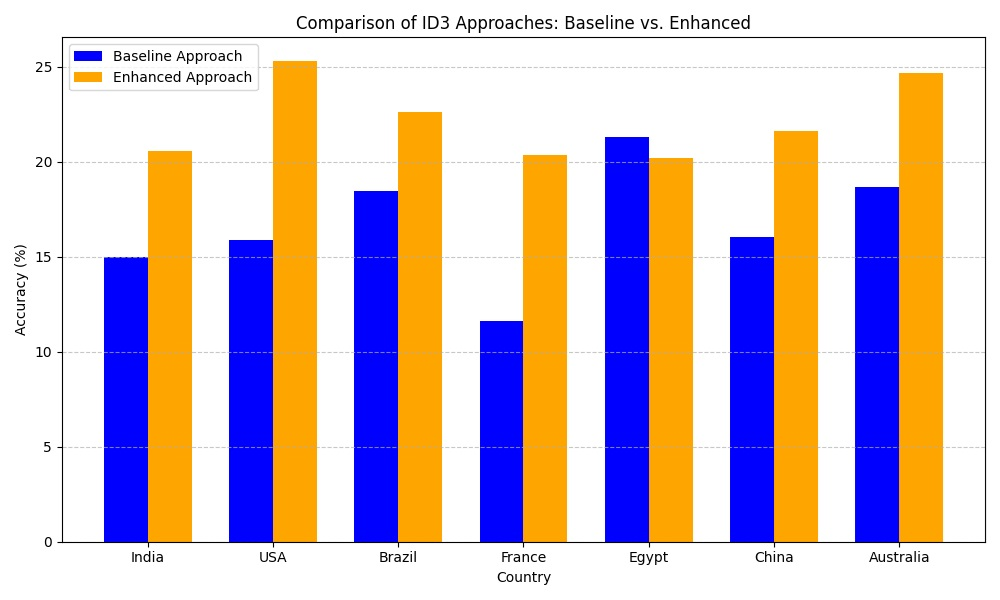
\includegraphics[width=0.8\textwidth]{comparation_id3_approaches.jpg}
    \caption{Accuracy Comparison Between Baseline and Enhanced ID3 Approaches}
    \label{fig:id3_comparison}
\end{figure}

\textbf{Key Insights:}
\begin{itemize}
    \item The enhanced approach consistently outperformed the baseline, demonstrating the importance of preprocessing techniques like discretization and parameter optimization.
    \item Despite improvements, the accuracy of the ID3 model remained relatively low (20\%-25\%), suggesting that further enhancements, such as additional feature engineering or the use of ensemble methods, may be needed.
\end{itemize}

\subsubsection{Conclusion}
The comparison between the baseline and enhanced approaches highlights the critical role of preprocessing in improving the performance of decision tree models. Discretization and hyperparameter tuning significantly improved accuracy and produced more reliable revenue hierarchies, making the enhanced approach preferable for this dataset.


\end{document}
